\hypertarget{tutorial-placing-obstacles-and-sensing-in-veranda}{%
\section{Tutorial: Placing Obstacles and Sensing in
Veranda}\label{tutorial-placing-obstacles-and-sensing-in-veranda}}

Assuming you've finished
\texttt{Tutorial\ 1\textless{}tutorial-1\textgreater{}}, you have a
little robot that can wander around aimlessly in an empty world. But one
of the most important parts of robotics is being able to take input from
sensors on your robot and react to your environment. This tutorial will
show you how to put some obstacles in the world with your robot and some
ways the sensors provided with Veranda can be used.

\hypertarget{part-1-making-obstacles}{%
\subsection{Part 1: Making obstacles}\label{part-1-making-obstacles}}

Having a robot that can drive around is fun, but eventually, you may
want to try to write code to make the robot avoid things it might run
into. The first step to doing that is having things for the robot to
hit. Veranda can load image files as a simulation, and turn them into
obstacles that robots can hit. To do this, choose the 'load simulation'
button, and find your image file. Make sure that all the obstacles you
want are in the image, because loading an image will clear your
simulation. This example image has a square that we can keep the robot
in, and some shapes in the middle for it to avoid.

\begin{figure}
\centering
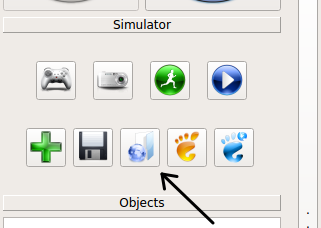
\includegraphics[width=0.75\textwidth,height=\textheight]{TutorialFigures/loadimage_button.*}
\caption{Use the 'Load Simulation' button to to load images as
obstacles}
\end{figure}

\begin{figure}
\centering

\includegraphics[width=0.75\textwidth,height=\textheight]{TutorialFigures/loadimage.*}
\caption{Example of the kind of image you might load. Make sure to get
all your obstacles in one picture!}
\end{figure}

Tip

Loading images in Veranda works best if they contain only black and
white pixels, with no other colors (including grey). If you do try to
load other images, you can play with the black/white threshold to get it
to turn out better.

Important

Veranda can load a number of different files as full simulations, make
sure you pick the correct file type in the file-choose dialog so that
you are able to select the file you want.

Once you choose an image, you will be presented with some import
options. The most important will be the size options, followed by the
threshold options. Veranda will report the size of the image, in pixels,
and you will have the option to set the pixel/m ratio, or and the image
size (in meters). Our little roomba has a radius of 2m, and the circle
obstacle in our image is 60 px in diameter, so if we set 30 px/m, the
robot will be the same size as that circle. Let's make it 10 px/m so the
robot is smaller than the circle.

\begin{figure}
\centering
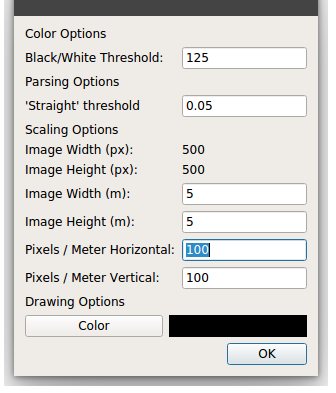
\includegraphics[width=0.5\textwidth,height=\textheight]{TutorialFigures/importoptions.*}
\caption{The image importing options}
\end{figure}

\begin{figure}
\centering
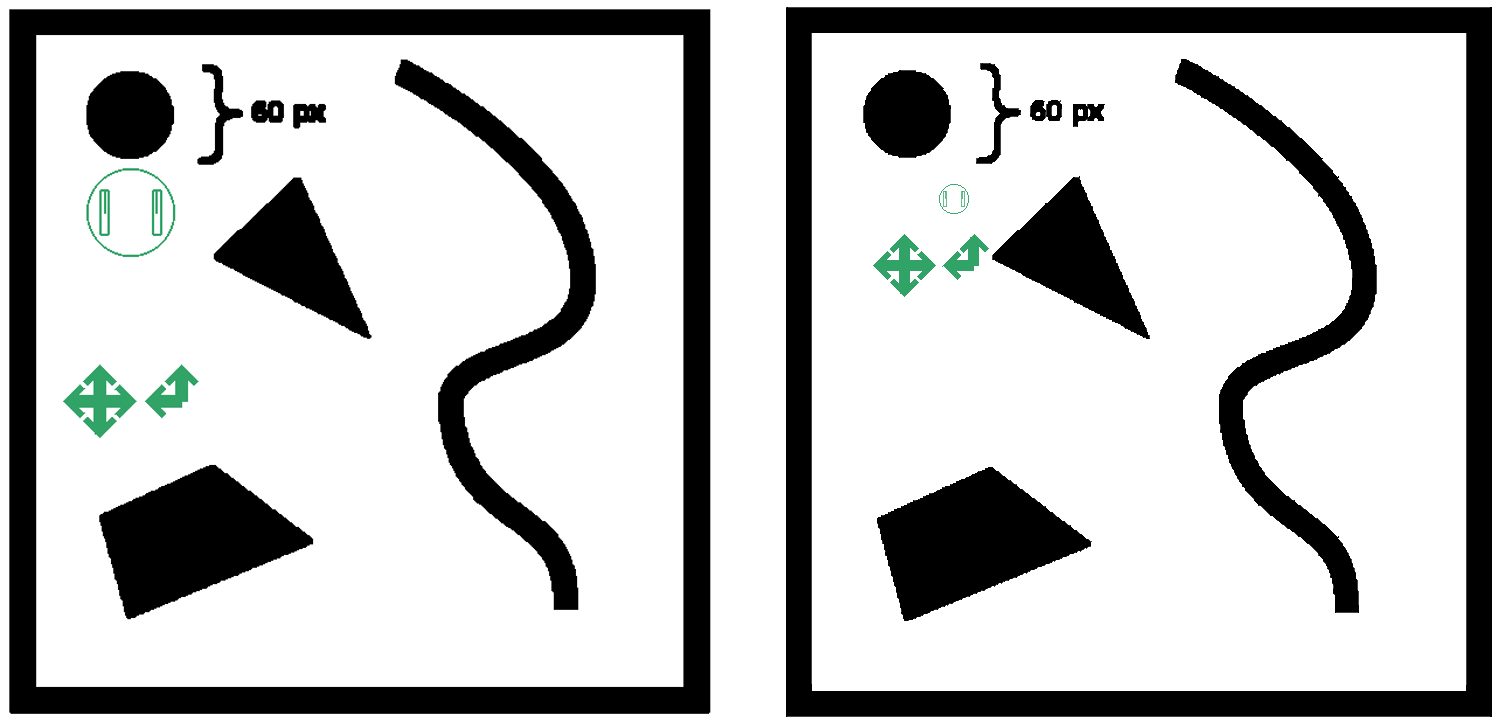
\includegraphics[width=1\textwidth,height=\textheight]{TutorialFigures/loadimage_scales.*}
\caption{Scaling the image to 30x30 px/m (left) and 10x10 px/m (right)}
\end{figure}

\hypertarget{part-2-did-it-crash}{%
\subsection{Part 2: Did it crash?}\label{part-2-did-it-crash}}

Now that there's something to hit, we want to know when the robot hits
it. To do this, we'll add a touch sensor to the robot; it will send
messages to the control script whenever it touches something.

In the editor, add a Touch Ring to your turtle bot. If you kept your
robot at the default size, you will not be able to see any difference,
because the touch ring is also a circle, and it defaults to 1m radius.

\begin{figure}
\centering
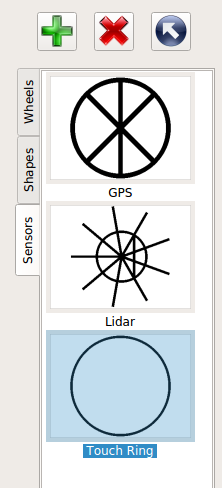
\includegraphics[width=0.5\textwidth,height=\textheight]{TutorialFigures/touchring.*}
\caption{Touch Ring is found under the sensors tab of the editor
toolbox}
\end{figure}

The touch ring represents a ring of bump sensors evenly spaced around
the robot; by default, the 'angle\_start' and 'angle\_end' properties,
which specify which part of the robot has the sensors, encompass the
entire chassis. Let's make there be 20 buttons them by setting the
property 'sensor\_count' to 20. Don't forget to set the ROS topic
property 'channels/output\_touches' to 'robot0/touches'.

\begin{figure}
\centering
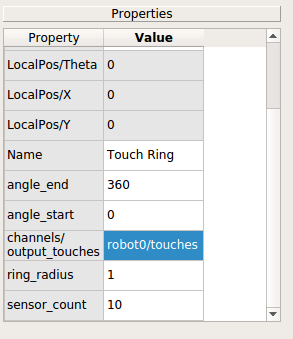
\includegraphics[width=0.5\textwidth,height=\textheight]{TutorialFigures/touchringproperties.*}
\caption{The properties we want to set for the touch ring}
\end{figure}

Tip

Don't have your robot loaded in the editor anymore? You can load it into
the editor from file!

\begin{figure}
\centering
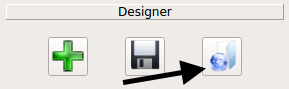
\includegraphics[width=0.5\textwidth,height=\textheight]{TutorialFigures/editorloadbutton.*}
\caption{The load button in the editor}
\end{figure}

Now, when your robot runs into a wall, you'll see a little circle appear
on the simulation representing the location of the touch sensor that was
triggered.

\begin{figure}
\centering
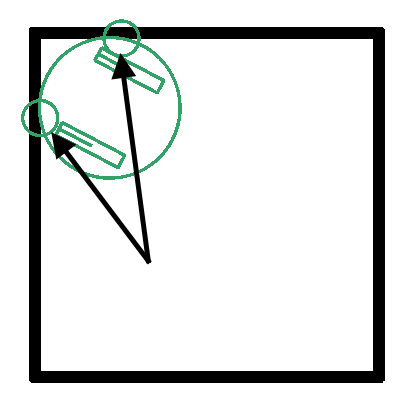
\includegraphics[width=0.5\textwidth,height=\textheight]{TutorialFigures/collisioncircles.*}
\caption{The indicators that your touch ring is sensing something}
\end{figure}

The last step is to set up a callback in your script to respond to this
stimulus. Let's modify \texttt{circle.py} for this one.

First, we have to import the message type that the touch ring publishes:
ByteMultiArray

\begin{Shaded}
\begin{Highlighting}[]
\ImportTok{from}\NormalTok{ std\_msgs.msg }\ImportTok{import}\NormalTok{ ByteMultiArray}
\end{Highlighting}
\end{Shaded}

Next, we create our callback function to handle this data. ROS callbacks
always have 1 parameter by default, and that is the message that was
sent. In the ROS std\_msg messages, each message has a \texttt{.data}
element which contains the actual information sent. Let's make a
callback that outputs the indexes of the buttons that were touched.
Because of how ROS handles the ByteMultiArray type in python, we have to
use the \texttt{struct::unpack()} function to get the data as a char
type.

\begin{Shaded}
\begin{Highlighting}[]
\ImportTok{from}\NormalTok{ struct }\ImportTok{import} \OperatorTok{*}
\KeywordTok{def}\NormalTok{ get\_hit(message):}
\NormalTok{    hits }\OperatorTok{=}\NormalTok{ message.data}

    \ControlFlowTok{for}\NormalTok{ i }\KeywordTok{in} \BuiltInTok{range}\NormalTok{(}\BuiltInTok{len}\NormalTok{(hits)):}
\NormalTok{        hit }\OperatorTok{=}\NormalTok{ unpack(}\StringTok{\textquotesingle{}b\textquotesingle{}}\NormalTok{, hits[i])[}\DecValTok{0}\NormalTok{]}

        \ControlFlowTok{if}\NormalTok{ hit }\OperatorTok{!=} \DecValTok{0}\NormalTok{: }
            \BuiltInTok{print}\NormalTok{(}\StringTok{"Touched on"}\NormalTok{, i)}
    \BuiltInTok{print}\NormalTok{(}\StringTok{"{-}{-}{-}{-}{-}{-}{-}{-}{-}{-}{-}{-}{-}{-}{-}{-}"}\NormalTok{)}
\end{Highlighting}
\end{Shaded}

Lastly, we set up a subscriber on the node which will listen to the
\texttt{robot0/touches} topic for ByteMultiArray messages and call the
callback function whenever a message comes in.

\begin{Shaded}
\begin{Highlighting}[]
\NormalTok{subtouches }\OperatorTok{=}\NormalTok{ node.create\_subscription(ByteMultiArray, }\StringTok{\textquotesingle{}robot0/touches\textquotesingle{}}\NormalTok{, get\_hit)}
\end{Highlighting}
\end{Shaded}

Now, if you load your little robot into that box and run this code, it
will hit the wall, and you'll see something like the following output

\begin{Shaded}
\begin{Highlighting}[]
\NormalTok{Touched on }\DecValTok{1}
\OperatorTok{{-}{-}{-}{-}{-}{-}{-}{-}{-}{-}{-}{-}{-}{-}{-}{-}}
\NormalTok{Touched on }\DecValTok{0}
\OperatorTok{{-}{-}{-}{-}{-}{-}{-}{-}{-}{-}{-}{-}{-}{-}{-}{-}}
\NormalTok{Touched on }\DecValTok{0}
\NormalTok{Touched on }\DecValTok{3}
\OperatorTok{{-}{-}{-}{-}{-}{-}{-}{-}{-}{-}{-}{-}{-}{-}{-}{-}}
\end{Highlighting}
\end{Shaded}

\begin{Shaded}
\begin{Highlighting}[]
\ImportTok{import}\NormalTok{ rclpy}
\ImportTok{from}\NormalTok{ rclpy.node }\ImportTok{import}\NormalTok{ Node}

\ImportTok{from}\NormalTok{ std\_msgs.msg }\ImportTok{import}\NormalTok{ Float32}

\ImportTok{from}\NormalTok{ std\_msgs.msg }\ImportTok{import}\NormalTok{ ByteMultiArray}
\ImportTok{from}\NormalTok{ struct }\ImportTok{import} \OperatorTok{*}

\KeywordTok{def}\NormalTok{ get\_hit(message):}
\NormalTok{    hits }\OperatorTok{=}\NormalTok{ message.data}

    \ControlFlowTok{for}\NormalTok{ i }\KeywordTok{in} \BuiltInTok{range}\NormalTok{(}\BuiltInTok{len}\NormalTok{(hits)):}
\NormalTok{        hit }\OperatorTok{=}\NormalTok{ unpack(}\StringTok{\textquotesingle{}b\textquotesingle{}}\NormalTok{, hits[i])[}\DecValTok{0}\NormalTok{]}

        \ControlFlowTok{if}\NormalTok{ hit }\OperatorTok{!=} \DecValTok{0}\NormalTok{: }
            \BuiltInTok{print}\NormalTok{(}\StringTok{"Touched on"}\NormalTok{, i)}
    \BuiltInTok{print}\NormalTok{(}\StringTok{"{-}{-}{-}{-}{-}{-}{-}{-}{-}{-}{-}{-}{-}{-}{-}{-}"}\NormalTok{)}

\NormalTok{rclpy.init()}
\NormalTok{node }\OperatorTok{=}\NormalTok{ Node(}\StringTok{"circle"}\NormalTok{)}

\NormalTok{publeft }\OperatorTok{=}\NormalTok{ node.create\_publisher(Float32, }\StringTok{\textquotesingle{}robot0/left\_wheel\textquotesingle{}}\NormalTok{)}
\NormalTok{pubright }\OperatorTok{=}\NormalTok{ node.create\_publisher(Float32, }\StringTok{\textquotesingle{}robot0/right\_wheel\textquotesingle{}}\NormalTok{)}

\NormalTok{subtouches }\OperatorTok{=}\NormalTok{ node.create\_subscription(ByteMultiArray, }\StringTok{\textquotesingle{}robot0/touches\textquotesingle{}}\NormalTok{, get\_hit)}

\NormalTok{msg }\OperatorTok{=}\NormalTok{ Float32()}

\NormalTok{msg.data }\OperatorTok{=} \FloatTok{5.0}
\NormalTok{publeft.publish(msg)}

\NormalTok{msg.data }\OperatorTok{=} \FloatTok{10.0}
\NormalTok{pubright.publish(msg)}

\NormalTok{rclpy.spin(node)}

\NormalTok{node.destroy\_node()}
\NormalTok{rclpy.shutdown()}
\end{Highlighting}
\end{Shaded}

\hypertarget{part-3-where-is-it}{%
\subsection{Part 3: Where is it?}\label{part-3-where-is-it}}

One of the most valuable pieces of information you can get is the
location of your robot. If you don't have a GPS, or some other
positioning system available, your robot will have to estimate it's
location based on what it sees. Fortunately, Veranda comes equipped with
a GPS sensor that you can use to get the absolute location of your
robot.

For this example, I added a GPS to my turtle robot, and set its output
channel to be robot0/gps.

\begin{figure}
\centering
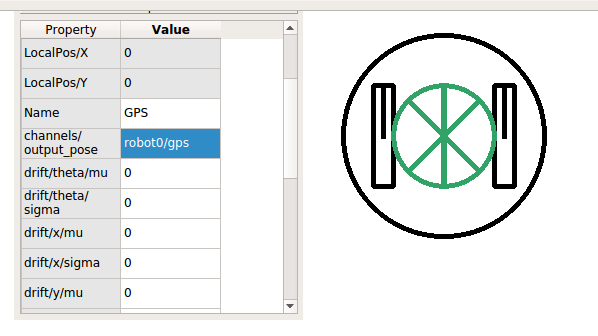
\includegraphics[width=0.8\textwidth,height=\textheight]{TutorialFigures/turtle_gps.*}
\caption{Turtle bot upgraded with a gps.}
\end{figure}

Now all we need to do to start listening to the robot locations is
subscribe to that topic and write a function to handle the ROS
\href{http://docs.ros.org/lunar/api/geometry_msgs/html/msg/Pose2D.html}{Pose2D}
message

Note

This link goes to the original ROS documentation; that's ok, a lot of
the built-in messages are the same as they were in ROS 1, just placed
under a different header directory

The Pose2D message contains 3 pieces of information: x, y, and theta -
the robot's location in the world and direction. Let's observe the
turtle's location as it drives in a circle.

First, we need to change our import statement to get the Pose2D message,
then we need to change our subscription to use that message.

\begin{Shaded}
\begin{Highlighting}[]
\ImportTok{from}\NormalTok{ geometry\_msgs.msg }\ImportTok{import}\NormalTok{ Pose2D}
\NormalTok{...}
\NormalTok{gps }\OperatorTok{=}\NormalTok{ node.create\_subscription(Pose2D, }\StringTok{\textquotesingle{}robot0/gps\textquotesingle{}}\NormalTok{, get\_position)}
\end{Highlighting}
\end{Shaded}

We also need to update our callback to handle the message. I set it up
to print the angle in degrees. Make sure you modulus the angle to get it
into the range you want, because it will just count up or down forever
if your robot spins.

\begin{Shaded}
\begin{Highlighting}[]
\ImportTok{import}\NormalTok{ math}
\KeywordTok{def}\NormalTok{ get\_position(message):}
    \BuiltInTok{print}\NormalTok{(}\StringTok{"Robot is at ("} \OperatorTok{+} \BuiltInTok{str}\NormalTok{(message.x) }\OperatorTok{+} \StringTok{","} \OperatorTok{+} \BuiltInTok{str}\NormalTok{(message.y) }\OperatorTok{+} \StringTok{") facing "} \OperatorTok{+} \BuiltInTok{str}\NormalTok{((message.theta}\OperatorTok{*}\DecValTok{180}\OperatorTok{/}\NormalTok{math.pi) }\OperatorTok{\%} \DecValTok{360}\NormalTok{) }\OperatorTok{+} \StringTok{" degrees"}\NormalTok{)}
    \BuiltInTok{print}\NormalTok{(}\StringTok{"{-}{-}{-}{-}{-}{-}{-}{-}{-}{-}{-}{-}{-}{-}{-}{-}"}\NormalTok{)}
\end{Highlighting}
\end{Shaded}

Other than those changes, our code is exactly the same as the code used
to print when the robot ran into something. This is what it outputs.

\begin{Shaded}
\begin{Highlighting}[]
\NormalTok{Robot }\KeywordTok{is}\NormalTok{ at (}\OperatorTok{{-}}\FloatTok{3.6408586502075195}\NormalTok{,}\OperatorTok{{-}}\FloatTok{0.10235483199357986}\NormalTok{) facing }\FloatTok{163.32569095773033}\NormalTok{ degrees}
\OperatorTok{{-}{-}{-}{-}{-}{-}{-}{-}{-}{-}{-}{-}{-}{-}{-}{-}}
\NormalTok{Robot }\KeywordTok{is}\NormalTok{ at (}\OperatorTok{{-}}\FloatTok{3.8731796741485596}\NormalTok{,}\OperatorTok{{-}}\FloatTok{0.5048621296882629}\NormalTok{) facing }\FloatTok{179.23729964819177}\NormalTok{ degrees}
\OperatorTok{{-}{-}{-}{-}{-}{-}{-}{-}{-}{-}{-}{-}{-}{-}{-}{-}}
\NormalTok{Robot }\KeywordTok{is}\NormalTok{ at (}\OperatorTok{{-}}\FloatTok{3.9862496852874756}\NormalTok{,}\OperatorTok{{-}}\FloatTok{0.9556393027305603}\NormalTok{) facing }\FloatTok{195.1489083386532}\NormalTok{ degrees}
\OperatorTok{{-}{-}{-}{-}{-}{-}{-}{-}{-}{-}{-}{-}{-}{-}{-}{-}}
\NormalTok{Robot }\KeywordTok{is}\NormalTok{ at (}\OperatorTok{{-}}\FloatTok{3.971405267715454}\NormalTok{,}\OperatorTok{{-}}\FloatTok{1.4201442003250122}\NormalTok{) facing }\FloatTok{211.06051702911464}\NormalTok{ degrees}
\OperatorTok{{-}{-}{-}{-}{-}{-}{-}{-}{-}{-}{-}{-}{-}{-}{-}{-}}
\NormalTok{Robot }\KeywordTok{is}\NormalTok{ at (}\OperatorTok{{-}}\FloatTok{3.8297839164733887}\NormalTok{,}\OperatorTok{{-}}\FloatTok{1.8627822399139404}\NormalTok{) facing }\FloatTok{226.97212571957607}\NormalTok{ degrees}
\OperatorTok{{-}{-}{-}{-}{-}{-}{-}{-}{-}{-}{-}{-}{-}{-}{-}{-}}
\NormalTok{Robot }\KeywordTok{is}\NormalTok{ at (}\OperatorTok{{-}}\FloatTok{3.572237491607666}\NormalTok{,}\OperatorTok{{-}}\FloatTok{2.2496349811553955}\NormalTok{) facing }\FloatTok{242.88373441003932}\NormalTok{ degrees}
\OperatorTok{{-}{-}{-}{-}{-}{-}{-}{-}{-}{-}{-}{-}{-}{-}{-}{-}}
\NormalTok{Robot }\KeywordTok{is}\NormalTok{ at (}\OperatorTok{{-}}\FloatTok{3.2185018062591553}\NormalTok{,}\OperatorTok{{-}}\FloatTok{2.551058292388916}\NormalTok{) facing }\FloatTok{258.79534310050076}\NormalTok{ degrees}
\OperatorTok{{-}{-}{-}{-}{-}{-}{-}{-}{-}{-}{-}{-}{-}{-}{-}{-}}
\NormalTok{Robot }\KeywordTok{is}\NormalTok{ at (}\OperatorTok{{-}}\FloatTok{2.795682191848755}\NormalTok{,}\OperatorTok{{-}}\FloatTok{2.743954658508301}\NormalTok{) facing }\FloatTok{274.7069517909622}\NormalTok{ degrees}
\OperatorTok{{-}{-}{-}{-}{-}{-}{-}{-}{-}{-}{-}{-}{-}{-}{-}{-}}
\NormalTok{Robot }\KeywordTok{is}\NormalTok{ at (}\OperatorTok{{-}}\FloatTok{2.336179733276367}\NormalTok{,}\OperatorTok{{-}}\FloatTok{2.8135430812835693}\NormalTok{) facing }\FloatTok{290.61856048142363}\NormalTok{ degrees}
\end{Highlighting}
\end{Shaded}

\begin{Shaded}
\begin{Highlighting}[]
\ImportTok{import}\NormalTok{ rclpy}
\ImportTok{from}\NormalTok{ rclpy.node }\ImportTok{import}\NormalTok{ Node}

\ImportTok{from}\NormalTok{ std\_msgs.msg }\ImportTok{import}\NormalTok{ Float32}

\ImportTok{from}\NormalTok{ geometry\_msgs.msg }\ImportTok{import}\NormalTok{ Pose2D}
\ImportTok{from}\NormalTok{ struct }\ImportTok{import} \OperatorTok{*}

\ImportTok{import}\NormalTok{ math}

\KeywordTok{def}\NormalTok{ get\_position(message):}
    \BuiltInTok{print}\NormalTok{(}\StringTok{"Robot is at ("} \OperatorTok{+} \BuiltInTok{str}\NormalTok{(message.x) }\OperatorTok{+} \StringTok{","} \OperatorTok{+} \BuiltInTok{str}\NormalTok{(message.y) }\OperatorTok{+} \StringTok{") facing "} \OperatorTok{+} \BuiltInTok{str}\NormalTok{((message.theta}\OperatorTok{*}\DecValTok{180}\OperatorTok{/}\NormalTok{math.pi) }\OperatorTok{\%} \DecValTok{360}\NormalTok{) }\OperatorTok{+} \StringTok{" degrees"}\NormalTok{)}
    \BuiltInTok{print}\NormalTok{(}\StringTok{"{-}{-}{-}{-}{-}{-}{-}{-}{-}{-}{-}{-}{-}{-}{-}{-}"}\NormalTok{)}

\NormalTok{rclpy.init()}
\NormalTok{node }\OperatorTok{=}\NormalTok{ Node(}\StringTok{"circle"}\NormalTok{)}

\NormalTok{publeft }\OperatorTok{=}\NormalTok{ node.create\_publisher(Float32, }\StringTok{\textquotesingle{}robot0/left\_wheel\textquotesingle{}}\NormalTok{)}
\NormalTok{pubright }\OperatorTok{=}\NormalTok{ node.create\_publisher(Float32, }\StringTok{\textquotesingle{}robot0/right\_wheel\textquotesingle{}}\NormalTok{)}

\NormalTok{gps }\OperatorTok{=}\NormalTok{ node.create\_subscription(Pose2D, }\StringTok{\textquotesingle{}robot0/gps\textquotesingle{}}\NormalTok{, get\_position)}

\NormalTok{msg }\OperatorTok{=}\NormalTok{ Float32()}

\NormalTok{msg.data }\OperatorTok{=} \FloatTok{5.0}
\NormalTok{publeft.publish(msg)}

\NormalTok{msg.data }\OperatorTok{=} \FloatTok{10.0}
\NormalTok{pubright.publish(msg)}

\NormalTok{rclpy.spin(node)}

\NormalTok{node.destroy\_node()}
\NormalTok{rclpy.shutdown()}
\end{Highlighting}
\end{Shaded}

Note

The GPS seems like a simple sensor, but it has a lot of options. In the
gps properties, you can properties for x, y, and theta to specify...

\begin{itemize}
\tightlist
\item
  Drift: How much error can accumulate on each time step
\item
  Noise: How far away from the drifted position can the reported
  position be
\item
  Probability: What is the probability {[}0, 1{]} that the value will
  not be invalid
\end{itemize}

For both Drift and Noise, you can specify the Sigma and Mu of the
Gaussian distribution used to pick values.

\hypertarget{part-4-whats-nearby}{%
\subsection{Part 4: What's nearby?}\label{part-4-whats-nearby}}

It's great that we can use a bump sensor to know when we hit something,
but wouldn't it be great if we could avoid crashing in the first place?
The LIDAR sensor allows for just that! It can simulate bouncing rays of
light across a range of angles to report how far away things are from
your robot. The message that the lidar publishes is the
\href{http://docs.ros.org/lunar/api/sensor_msgs/html/msg/LaserScan.html}{LaserScan}
message.

Let's upgrade our turtle again, and put it somewhere that the lidar will
sense something.

\begin{figure}
\centering
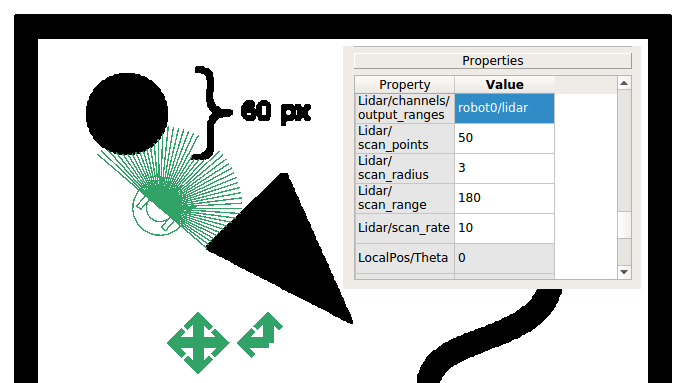
\includegraphics[width=0.8\textwidth,height=\textheight]{TutorialFigures/turtle_lidar.*}
\caption{Turtle bot upgraded with a lidar, sensing some obstacles. I set
my lidar to report on the robot0/lidar channel. It is sensing 180
degrees in front of it, with 50 rays that go 3 meters at max.}
\end{figure}

Note

In that image, the lines for the lidar had been updated during
simulation. Right after you place the robot, they won't change to
reflect what's around them until you press 'play'.

Once again, changing our existing code to use the new message is pretty
easy; the hard part is understanding the LaserScan message. This code
will make the robot spin slowly in place, and it will print the message
as-is when it arrives.

\begin{Shaded}
\begin{Highlighting}[]
\ImportTok{import}\NormalTok{ rclpy}
\ImportTok{from}\NormalTok{ rclpy.node }\ImportTok{import}\NormalTok{ Node}

\ImportTok{from}\NormalTok{ std\_msgs.msg }\ImportTok{import}\NormalTok{ Float32}

\ImportTok{from}\NormalTok{ sensor\_msgs.msg }\ImportTok{import}\NormalTok{ LaserScan}
\ImportTok{from}\NormalTok{ struct }\ImportTok{import} \OperatorTok{*}

\ImportTok{import}\NormalTok{ math}

\KeywordTok{def}\NormalTok{ get\_position(message):}
    \BuiltInTok{print}\NormalTok{(message)}
    \BuiltInTok{print}\NormalTok{(}\StringTok{"{-}{-}{-}{-}{-}{-}{-}{-}{-}{-}{-}{-}{-}{-}{-}{-}"}\NormalTok{)}

\NormalTok{rclpy.init()}
\NormalTok{node }\OperatorTok{=}\NormalTok{ Node(}\StringTok{"circle"}\NormalTok{)}

\NormalTok{publeft }\OperatorTok{=}\NormalTok{ node.create\_publisher(Float32, }\StringTok{\textquotesingle{}robot0/left\_wheel\textquotesingle{}}\NormalTok{)}
\NormalTok{pubright }\OperatorTok{=}\NormalTok{ node.create\_publisher(Float32, }\StringTok{\textquotesingle{}robot0/right\_wheel\textquotesingle{}}\NormalTok{)}

\NormalTok{gps }\OperatorTok{=}\NormalTok{ node.create\_subscription(LaserScan, }\StringTok{\textquotesingle{}robot0/lidar\textquotesingle{}}\NormalTok{, get\_position)}

\NormalTok{msg }\OperatorTok{=}\NormalTok{ Float32()}

\NormalTok{msg.data }\OperatorTok{=} \FloatTok{0.5}
\NormalTok{publeft.publish(msg)}

\NormalTok{msg.data }\OperatorTok{=} \OperatorTok{{-}}\FloatTok{0.5}
\NormalTok{pubright.publish(msg)}

\NormalTok{rclpy.spin(node)}

\NormalTok{node.destroy\_node()}
\NormalTok{rclpy.shutdown()}
\end{Highlighting}
\end{Shaded}

Let's take a look at one of the LaserScan messages

\begin{Shaded}
\begin{Highlighting}[]
\NormalTok{sensor\_msgs.msg.LaserScan(}
\NormalTok{    header}\OperatorTok{=}\NormalTok{std\_msgs.msg.Header(}
\NormalTok{        stamp}\OperatorTok{=}\NormalTok{builtin\_interfaces.msg.Time(sec}\OperatorTok{=}\DecValTok{0}\NormalTok{, nanosec}\OperatorTok{=}\DecValTok{0}\NormalTok{), }
\NormalTok{        frame\_id}\OperatorTok{=}\StringTok{\textquotesingle{}\textquotesingle{}}\NormalTok{), }
\NormalTok{    angle\_min}\OperatorTok{={-}}\FloatTok{1.5707963705062866}\NormalTok{, }
\NormalTok{    angle\_max}\OperatorTok{=}\FloatTok{1.5707963705062866}\NormalTok{, }
\NormalTok{    angle\_increment}\OperatorTok{=}\FloatTok{0.06411413848400116}\NormalTok{, }
\NormalTok{    time\_increment}\OperatorTok{=}\FloatTok{0.0}\NormalTok{, }
\NormalTok{    scan\_time}\OperatorTok{=}\FloatTok{0.10000000149011612}\NormalTok{, }
\NormalTok{    range\_min}\OperatorTok{=}\FloatTok{2.1359217166900635}\NormalTok{, }
\NormalTok{    range\_max}\OperatorTok{=}\FloatTok{2.844834089279175}\NormalTok{, }
\NormalTok{    ranges}\OperatorTok{=}\NormalTok{[inf, inf, inf, inf, inf, inf, inf, inf, inf, inf, }
            \FloatTok{2.2153570652008057}\NormalTok{, }\FloatTok{2.213566303253174}\NormalTok{, }\FloatTok{2.2417705059051514}\NormalTok{, }\FloatTok{2.280193567276001}\NormalTok{, }
            \FloatTok{2.3296966552734375}\NormalTok{, }\FloatTok{2.391442060470581}\NormalTok{, }\FloatTok{2.4669628143310547}\NormalTok{, }\FloatTok{2.5582637786865234}\NormalTok{, }
            \FloatTok{2.7111518383026123}\NormalTok{, }\FloatTok{2.844834089279175}\NormalTok{, inf, inf, inf, inf, inf, inf, inf, inf, }
\NormalTok{            inf, inf, inf, inf, inf, inf, }\FloatTok{2.3573288917541504}\NormalTok{, }\FloatTok{2.236565351486206}\NormalTok{, }\FloatTok{2.1359217166900635}\NormalTok{, }
\NormalTok{            inf, inf, inf, inf, inf, inf, inf, inf, }\FloatTok{2.6468541622161865}\NormalTok{, }\FloatTok{2.440544605255127}\NormalTok{, }
            \FloatTok{2.3114850521087646}\NormalTok{, }\FloatTok{2.2470221519470215}\NormalTok{, }\FloatTok{2.1885221004486084}\NormalTok{], }
\NormalTok{    intensities}\OperatorTok{=}\NormalTok{[])}
\end{Highlighting}
\end{Shaded}

There's a lot here to unpack, so let's go one item at a time

\begin{itemize}
\tightlist
\item
  header: Every ROS message has a header stating the message time and
  the message's id. These are not populated by the Veranda Lidar.
\item
  angle\_min/maximum\_angle: Bounding range (radians) of the scan,
  relative to the lidar. Our lidar has a range of 180 degrees, so it
  goes from -90 to +90, or -pi to +pi.
\item
  angle\_increment: Number of radians between each scan point
\item
  time\_increment: Time taken between each scan point. Since Veranda is
  a simulation, we can pause the world and scan it, resulting in
  instantaneous information
\item
  scan\_time: Total time taken to do the scan. This lidar is set to
  output at 10hz, so that's what it reports.
\item
  range\_min/range\_max: Minimum and Maximum distance (meters) seen by
  the lidar.
\item
  ranges: The actual distances seen by the lidar, 1 per scan point. They
  are reported from minimum angle to maximum. Locations where nothing
  was seen report infinity.
\item
  intensities: Some lidars (not Veranda's simulation) report the
  intensity of the light at each point
\end{itemize}

\hypertarget{part-5-how-fast-is-it-going}{%
\subsection{Part 5: How fast is it
going?}\label{part-5-how-fast-is-it-going}}

The last sensor we're going to discuss here is the encoder. Encoders are
devices that can be used to measure the angular velocity of an axle.
While real encoders might report frequency of a spinning stripe in front
of a sensor, the encoders included in Veranda just report angular
velocity. They are attached by default to both the fixed wheel type and
Ackermann steering weels type. Just add a wheel to get an encoder.
However, until you set the output topic for an encoder, it will do
nothing.

Encoders return a single value, the angular velocity of the wheel in
radians/second. If we set the output channels for our encoders, and add
a little bit of noise, we can see how the noise affects the output while
the robot drives in a circle.

\begin{Shaded}
\begin{Highlighting}[]
\ImportTok{import}\NormalTok{ rclpy}
\ImportTok{from}\NormalTok{ rclpy.node }\ImportTok{import}\NormalTok{ Node}

\ImportTok{from}\NormalTok{ std\_msgs.msg }\ImportTok{import}\NormalTok{ Float32}

\ImportTok{from}\NormalTok{ struct }\ImportTok{import} \OperatorTok{*}

\ImportTok{import}\NormalTok{ math}

\NormalTok{left\_speed, right\_speed }\OperatorTok{=} \DecValTok{0}\NormalTok{, }\DecValTok{0}

\KeywordTok{def}\NormalTok{ output():}
    \BuiltInTok{print}\NormalTok{(}\StringTok{"Wheel speeds: "} \OperatorTok{+} \BuiltInTok{str}\NormalTok{(left\_speed) }\OperatorTok{+} \StringTok{" {-} "} \OperatorTok{+} \BuiltInTok{str}\NormalTok{(right\_speed))}
    \BuiltInTok{print}\NormalTok{(}\StringTok{"{-}{-}{-}{-}{-}{-}{-}{-}{-}{-}{-}{-}{-}{-}{-}{-}"}\NormalTok{)}

\KeywordTok{def}\NormalTok{ get\_left(message):}
    \KeywordTok{global}\NormalTok{ left\_speed}

\NormalTok{    left\_speed }\OperatorTok{=}\NormalTok{ message.data}
\NormalTok{    output()}

\KeywordTok{def}\NormalTok{ get\_right(message):}
    \KeywordTok{global}\NormalTok{ right\_speed}

\NormalTok{    right\_speed }\OperatorTok{=}\NormalTok{ message.data}
\NormalTok{    output()}

\NormalTok{rclpy.init()}
\NormalTok{node }\OperatorTok{=}\NormalTok{ Node(}\StringTok{"circle"}\NormalTok{)}

\NormalTok{publeft }\OperatorTok{=}\NormalTok{ node.create\_publisher(Float32, }\StringTok{\textquotesingle{}robot0/left\_wheel\textquotesingle{}}\NormalTok{)}
\NormalTok{pubright }\OperatorTok{=}\NormalTok{ node.create\_publisher(Float32, }\StringTok{\textquotesingle{}robot0/right\_wheel\textquotesingle{}}\NormalTok{)}

\NormalTok{subleft }\OperatorTok{=}\NormalTok{ node.create\_subscription(Float32, }\StringTok{\textquotesingle{}robot0/left\_encoder\textquotesingle{}}\NormalTok{, get\_left)}
\NormalTok{subright }\OperatorTok{=}\NormalTok{ node.create\_subscription(Float32, }\StringTok{\textquotesingle{}robot0/right\_encoder\textquotesingle{}}\NormalTok{, get\_right)}

\NormalTok{msg }\OperatorTok{=}\NormalTok{ Float32()}

\NormalTok{msg.data }\OperatorTok{=} \FloatTok{5.0}
\NormalTok{publeft.publish(msg)}

\NormalTok{msg.data }\OperatorTok{=} \FloatTok{10.0}
\NormalTok{pubright.publish(msg)}

\NormalTok{rclpy.spin(node)}

\NormalTok{node.destroy\_node()}
\NormalTok{rclpy.shutdown()}
\end{Highlighting}
\end{Shaded}

\begin{Shaded}
\begin{Highlighting}[]
\OperatorTok{{-}{-}{-}{-}{-}{-}{-}{-}{-}{-}{-}{-}{-}{-}{-}{-}}
\NormalTok{Wheel speeds: }\FloatTok{2.6641697883605957} \OperatorTok{{-}} \FloatTok{7.652131080627441}
\OperatorTok{{-}{-}{-}{-}{-}{-}{-}{-}{-}{-}{-}{-}{-}{-}{-}{-}}
\NormalTok{Wheel speeds: }\FloatTok{2.6641697883605957} \OperatorTok{{-}} \FloatTok{10.325849533081055}
\OperatorTok{{-}{-}{-}{-}{-}{-}{-}{-}{-}{-}{-}{-}{-}{-}{-}{-}}
\NormalTok{Wheel speeds: }\FloatTok{5.337887287139893} \OperatorTok{{-}} \FloatTok{10.325849533081055}
\OperatorTok{{-}{-}{-}{-}{-}{-}{-}{-}{-}{-}{-}{-}{-}{-}{-}{-}}
\NormalTok{Wheel speeds: }\FloatTok{3.404207706451416} \OperatorTok{{-}} \FloatTok{10.325849533081055}
\OperatorTok{{-}{-}{-}{-}{-}{-}{-}{-}{-}{-}{-}{-}{-}{-}{-}{-}}
\NormalTok{Wheel speeds: }\FloatTok{3.404207706451416} \OperatorTok{{-}} \FloatTok{8.392169952392578}
\OperatorTok{{-}{-}{-}{-}{-}{-}{-}{-}{-}{-}{-}{-}{-}{-}{-}{-}}
\end{Highlighting}
\end{Shaded}
